\documentclass[12pt]{article}
\usepackage{graphicx}
\usepackage[none]{hyphenat}
\usepackage{graphicx}
\usepackage{listings}
\usepackage[english]{babel}
\usepackage{graphicx}
\usepackage{caption} 
\usepackage{booktabs}
\usepackage{array}
\usepackage{amssymb} % for \because
\usepackage{amsmath}   % for having text in math mode
\usepackage{extarrows} % for Row operations arrows
\usepackage{listings}
\usepackage[utf8]{inputenc}
\lstset{
  frame=single,
  breaklines=true
}
\usepackage{hyperref}
  
%Following 2 lines were added to remove the blank page at the beginning
\usepackage{atbegshi}% http://ctan.org/pkg/atbegshi
\AtBeginDocument{\AtBeginShipoutNext{\AtBeginShipoutDiscard}}


%New macro definitions
\newcommand{\mydet}[1]{\ensuremath{\begin{vmatrix}#1\end{vmatrix}}}
\providecommand{\brak}[1]{\ensuremath{\left(#1\right)}}
\newcommand{\solution}{\noindent \textbf{Solution: }}
\newcommand{\myvec}[1]{\ensuremath{\begin{pmatrix}#1\end{pmatrix}}}
\providecommand{\norm}[1]{\left\lVert#1\right\rVert}
\providecommand{\abs}[1]{\left\vert#1\right\vert}
\let\vec\mathbf

\begin{document}

\begin{center}
\title{\textbf{LINE}}
\date{\vspace{-5ex}} %Not to print date automatically
\maketitle
\end{center}

\section{11$^{th}$ Maths - EXERCISE-10.4}
\begin{enumerate}
\item What are the points on the y-axis whose distance from the line $\frac{x}{3}+\frac{y}{4}=1$ is 4 units.
\end{enumerate}
\section{SOLUTION}
Given line equation is
\begin{align}
\frac{x}{3}+\frac{y}{4}&=1\\
\myvec{4x+3y-12}&=0\\
\vec{n}&=\myvec{4\\3}\\
c&=12
\end{align}
The distance of the line from y-axis
\begin{align}
d&=\frac{\vec{n}^\top\vec{P}-c}{\abs{n}}\\
\implies\pm4&=\frac{\myvec{4& 3}\myvec{0\\ y}-12}{5}\\
\implies\pm4&=\frac{\myvec{0\\ 3y}-12}{5}\\
\implies\pm20&=3y-12\\
\implies 3y&=20\pm12\\
\implies y= \frac{32}{3}\text{ or }y=\frac{-8}{3}
\end{align}

\section{FIGURE}
\begin{figure}[h]
\centering
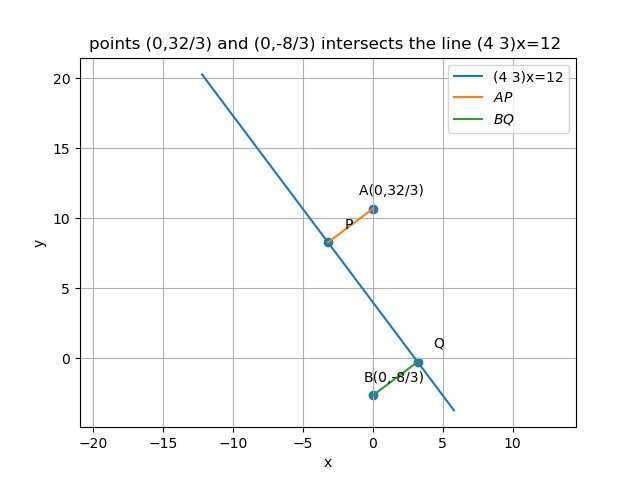
\includegraphics[width=\columnwidth]{fig.png}
\caption{line}
		\label{fig:Figure}
\end{figure}
\end{document}